Le Snake Cube (ou cube serpent en français) est un casse-tête géométrique à trois dimensions appartenant à la famille des casse-tête mécaniques. Cette famille, dont fait parti le Rubik’s Cube, recouvre l’ensemble des jeux de réflexion basés sur la manipulation d’un objet tridimensionnel, afin de lui donner un agencement précis.

\begin{figure}[h]
 \centering
 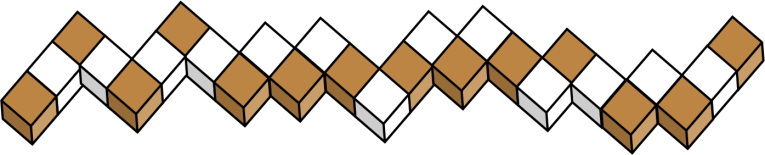
\includegraphics[scale=0.5,keepaspectratio=true]{img/snakeCubeFlat.png}
 \caption{Snake Cube déplié}
 \label{snakeFlat}
\end{figure}

Ce casse-tête se présente généralement comme une succession de 27 petits cubes en bois, reliés les uns aux autres par un fil élastique qui les traverse de part en part. Lorsque tous les cubes sont mis sur le même plan, la forme du puzzle s’apparente à un serpent  (Figure~\ref{snakeFlat}). Pour résoudre le puzzle, il faut manier le serpent afin de le ramener à une forme entièrement cubique telle que présentée ci-dessous (Figure~\ref{snakeSolved}). Dans la suite de cette partie et pour éviter les ambiguïtés, les petits cubes qui forment le serpent seront appelés \textbf{unités} tandis que le mot cube désignera plutôt le volume final visible sur la figure~\ref{snakeSolved}.

\begin{figure}[h]
 \centering
 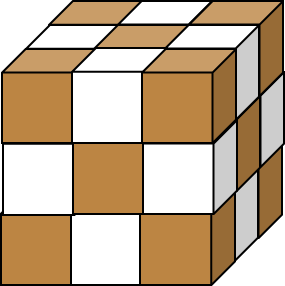
\includegraphics[scale=0.5,keepaspectratio=true]{img/snakeCubeSolved.png}
 \caption{Snake Cube résolu}
 \label{snakeSolved}
\end{figure}

\newpage Comme mentionné précédemment, les unités sont reliées entre elles ce qui les rend totalement indissociables. Ainsi, les manipulations pouvant être effectuées sur le puzzle sont réduites à des rotations. La Figure~\ref{snakeMove} illustre une manipulation réalisée sur le serpent présenté figure~\ref{snakeFlat}. De plus, on remarque que les rotations conduisant à modifier la forme de la figure s’effectuent toujours au niveau des coins du serpent. Cette particularité sera notamment exploitée lorsque l’on traitera de la résolution du casse-tête.

\begin{figure}[h]
 \centering
 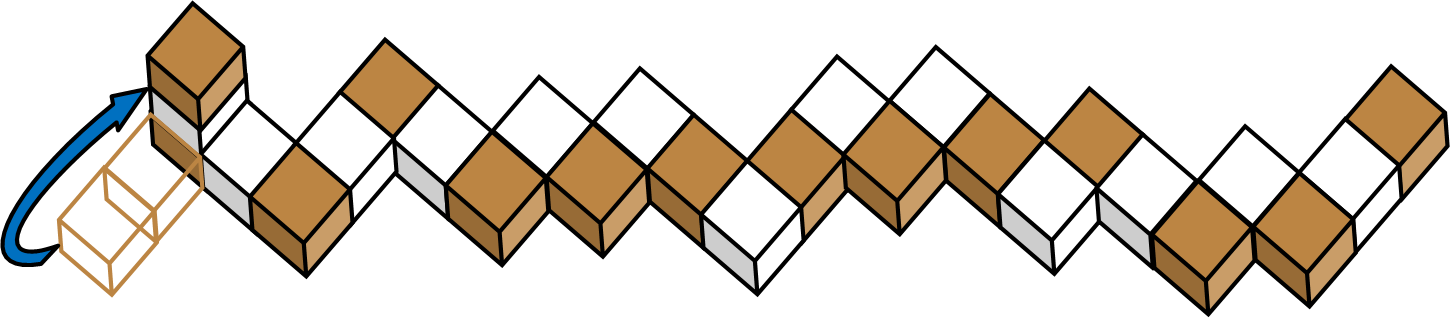
\includegraphics[scale=0.3,keepaspectratio=true]{img/snakeCubeMove.png}
 \caption{Exemple de manipulation du Snake Cube}
 \label{snakeMove}
\end{figure}

Notons également  que pour une figure finale donnée (ici une cube 3x3x3), il existe une multitude de formes de serpents correspondantes. Les serpents les plus connus seront listés en annexe de ce document, associés à leurs spécificités (difficulté, nombre de solutions, temps de calcul correspondant). De manière moins classique, on trouve aussi dans le commerce des serpents permettant de réaliser des cubes 4x4x4. À notre connaissance il n’existe pas de casse-tête correspondant à des Snake Cubes de tailles supérieures.